% This file was created by tikzplotlib v0.9.2.
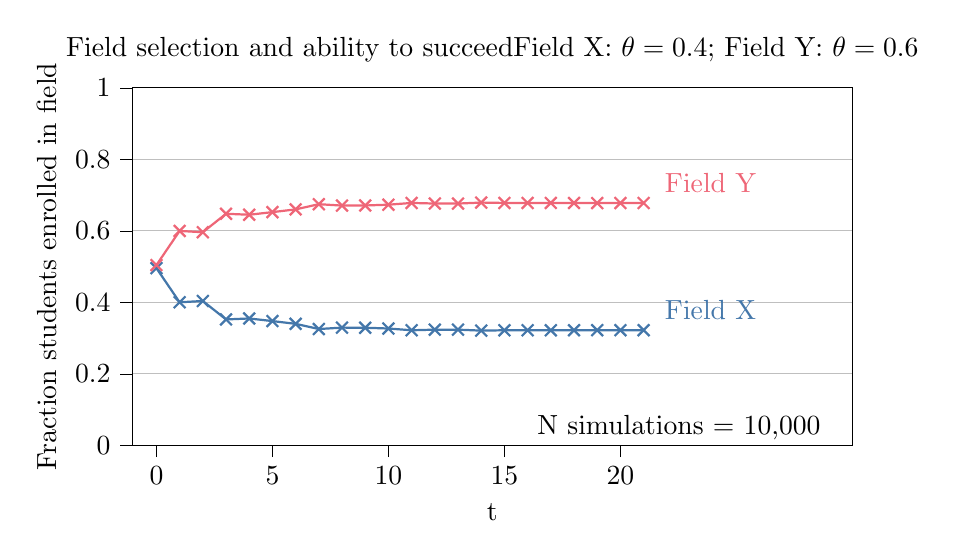
\begin{tikzpicture}

\definecolor{color0}{rgb}{0.266666666666667,0.466666666666667,0.666666666666667}
\definecolor{color1}{rgb}{0.933333333333333,0.4,0.466666666666667}

\begin{axis}[
height=6.121302808757603cm,
tick align=outside,
tick pos=left,
title={Field selection and ability to succeed \\ Field X: \(\displaystyle \theta = 0.4\); Field Y: \(\displaystyle \theta = 0.6\)},
width=10.729849cm,
x grid style={white!69.0196078431373!black},
xlabel={t},
xmin=-1.05, xmax=30,
xtick style={color=black},
xtick={0,5,10,15,20},
xticklabels={\(\displaystyle 0\),\(\displaystyle 5\),\(\displaystyle 10\),\(\displaystyle 15\),\(\displaystyle 20\)},
ylabel={Fraction students enrolled in field},
ymajorgrids,
ymin=0, ymax=1,
ytick style={color=black},
ytick={0,0.2,0.4,0.6,0.8,1},
yticklabels={\(\displaystyle 0\),\(\displaystyle 0.2\),\(\displaystyle 0.4\),\(\displaystyle 0.6\),\(\displaystyle 0.8\),\(\displaystyle 1\)}
]
\addplot [thick, color0, mark=x, mark size=3, mark options={solid}]
table {%
0 0.4957
1 0.4002
2 0.4038
3 0.3522
4 0.3549
5 0.3476
6 0.3399
7 0.3254
8 0.3293
9 0.329
10 0.3268
11 0.3219
12 0.3236
13 0.3236
14 0.3209
15 0.3219
16 0.3219
17 0.3219
18 0.322
19 0.3222
20 0.3222
21 0.3222
};
\addplot [thick, color1, mark=x, mark size=3, mark options={solid}]
table {%
0 0.5043
1 0.5998
2 0.5962
3 0.6478
4 0.6451
5 0.6524
6 0.6601
7 0.6746
8 0.6707
9 0.671
10 0.6732
11 0.6781
12 0.6764
13 0.6764
14 0.6791
15 0.6781
16 0.6781
17 0.6781
18 0.678
19 0.6778
20 0.6778
21 0.6778
};
\draw (axis cs:21.5,0.3522) node[
  anchor=base west,
  text=color0,
  rotate=0.0
]{Field X};
\draw (axis cs:21.5,0.7078) node[
  anchor=base west,
  text=color1,
  rotate=0.0
]{Field Y};
\draw (axis cs:16,0.03) node[
  anchor=base west,
  text=black,
  rotate=0.0
]{N simulations = 10,000};
\end{axis}

\end{tikzpicture}
